\documentclass[conference]{IEEEtran}
\IEEEoverridecommandlockouts
% The preceding line is only needed to identify funding in the first footnote. If that is unneeded, please comment it out.
\usepackage{cite}
\usepackage{amsmath,amssymb,amsfonts}
\usepackage{algorithmic}
\usepackage{graphicx}
\usepackage{textcomp}
\usepackage{xcolor}
\usepackage[hyphens]{url}
\def\BibTeX{{\rm B\kern-.05em{\sc i\kern-.025em b}\kern-.08em
    T\kern-.1667em\lower.7ex\hbox{E}\kern-.125emX}}
\begin{document}

\title{Scaling Data Menggunakan Metode MinMax Scaler\\
}

\author{\IEEEauthorblockN{1\textsuperscript{st} Aditya Rahman}
\IEEEauthorblockA{\textit{Teknik Elektro} \\
\textit{Universitas Negeri Malang}\\
Malang, Indonesia \\
aditya@klim.or.id}

\and
\IEEEauthorblockN{2\textsuperscript{nd} Galih Hadi Wibowo}
\IEEEauthorblockA{\textit{Teknik Elektro} \\
\textit{Universitas Negeri Malang}\\
Malang, Indonesia \\
hadigalih@gmail.com}
}

\maketitle

\begin{abstract}
Feature Scaling adalah metode yang digunakan untuk normalisasi rentang dari variabel independen atau data dari suatu fitur. Pada pemrosesan data dikenal sebagai Normalisasi dan umumnya dilakukan pada pra-proses data. MinMax Scaling merupakan metode paling sederhana dalam melakukan scaling sebuah variabel menjadi rentang tertentu. Penggunaan Scaling pada algoritma Naive Bayes secara teori tidak memiliki dampak yang signifikan, namun pada pengujian didapatkan hasil bahwa Penggunaan Scaling menghasilkan waktu Training lebih cepat 45\%, akurasi lebih tinggi sebesar 11\% dan presisi lebih besar 25\% dibanding penggunaan data tanpa Scaling pada algoritma yang sama pada saaat melakukan CrossValidation. 
\end{abstract}

\begin{IEEEkeywords}
Scaling, MinMax Scaler
\end{IEEEkeywords}

\section{Pendahuluan}

\subsection{Latar Belakang}
Dataset ini berasal dari National Institute of Diabetes and DIgestive and Kidney Diseases. PIMA INDIAN Diabetes adalah penduduk asli amerika hidup di Arizona. Kecenderungan genetik yang dialami memungkinkan kelompok ini untuk bertahan hidup secara normal untuk diet karbohidrat yang buruk selama bertahun-tahun. Beberapa tahun ini, dikarenakan transisi yang mendadak dari makanan pertanian tradisional menjadi makanan olahan, bersamaan dengan menurunnya aktivitas fisik, membuat mereka menjadi frekuensi tertinggi yang mengalami diabetes tipe 2 dan karena alasan ini mereka mejadi subjek dari berbagai macam studi. 

Dataset berisi berbagai variabel prediksi medis dan satu variabel target "Outcome", jika output 1 maka diabetes, jika 0 maka tidak diabetes. Variabel prediksi medis berisi jumlah kehamilan yang dialami pasien, BMI mereka, level insulin, umur, dan seterusnya.

Dataset ini mengandung nilai yang sangat bervariasi pada fitur Glukosa, memiliki nilai minimum 0, nilai maksimum 199, dan variance 1022. Sedangkan metode Naive Bayes Gaussian secara teori tidak memiliki pengaruh signifikan pada feature scaling karena Naive Bayes secara desain dapat menangani algoritma seperti Linear Discriminant Analysis. 

Scaling memiliki pengaruh yang signifikan pada algoritma yang sensitif pada jarak seperti algoritma KMeans, karna itu data harus dilakukan scale agar tiap fitur memiliki bobot yang equal.

Pengujian menggunakan MinMax Scale karna metode ini mudah diterapkan untuk data yang tidak memiliki begitu banyak outlier sehingga hanya untuk melakukan normalisasi MinMax cukup untuk dataset ini. 

\subsection{Tujuan}
Untuk mencari dampak dari penggunaan "Scaling" pada waktu eksekusi, akurasi prediksi, preisisi dari model pada Gaussian Naive Bayes dan Support Vector Machine Support Vector Classification.

\section{Metode Scaling}
Juga dikenal sebagai min-max normalisasi, adalah metode paling sederhana untuk melakukan scaling. Mengubah features dengan melakukan scaling pada tiap instances menjadi range nilai tertentu. Pada artikel ini menerapkan scaling dengan range 0 hingga 1. MinMaxScale juga dapat memiliki output berupa range tertentu misal 1 hingga 3 dan seterusnya. 

\begin{equation}
\label{minmax_scaler_formula}
X' = a + 
\frac{(X_1-min(X))(b-a)}{max(X)-min(X)}
\end{equation}

Dengan:

$a$ : range bawah

$b$ : range atas

$X_i$ : value dari suatu features

$min(X)$ : nilai minimum dari features X

$max(X)$ : nilai maksimum dari features X

\section{Penerapan}
Data PAMA INDIAN sebelum diterapkan MinMax Scaler jika ditampilkan seperti berikut ini

\begin{figure}[htbp]
	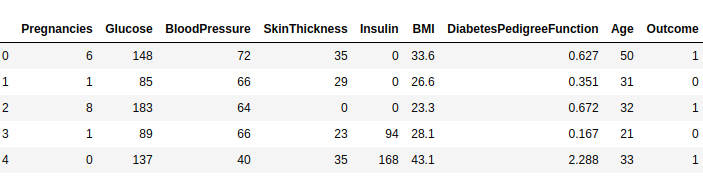
\includegraphics[width=\linewidth]{img/sebelumminmax.png}
	\caption{Data sebelum menggunakan MinMax Scaler.}
\end{figure}

Setelah diterapkan MinMax Scaler pada features Glucose

\begin{figure}[htbp]
	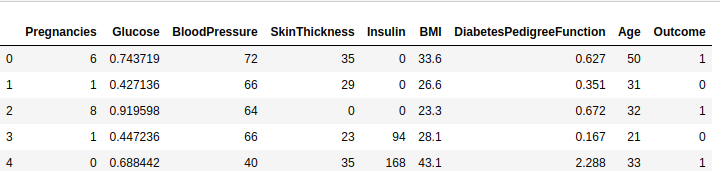
\includegraphics[width=\linewidth]{img/sesudahminmax.png}
	\caption{Data sesudah menggunakan MinMax Scaler.}
\end{figure}

Penerapan menggunakan modul MinMaxScaler dari library sklearn.preprocessing

Visualisasi data setelah diberlakukan Scaling pada features Glucose dan Pregnancies. Dilihat dari plot sebelah kiri bahwa kedua feaures tersebut memiliki rentang nilai yang berbeda, namun pada plot sebelah kanan data tersebut telah diterapkan MinMaxScale memiliki plot yang serupa karna memiliki rentang nilai yang serupa. 

\begin{figure}[htbp]
	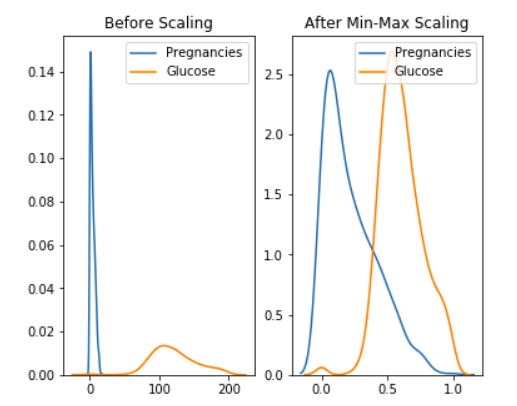
\includegraphics[width=\linewidth]{img/graph.png}
	\caption{Menggunakan module sklearn.preprocessing.}
\end{figure}

\begin{figure}[htbp]
	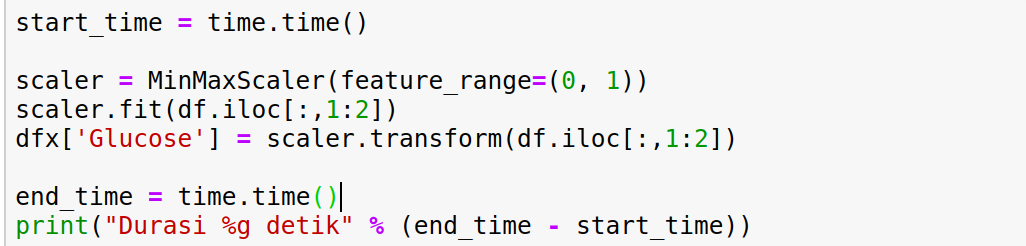
\includegraphics[width=\linewidth]{img/sklearn_preprocessing.png}
	\caption{Menggunakan module sklearn.preprocessing.}
\end{figure}

Durasi yang diperlukan untuk transformasi features Glucose

\begin{figure}[htbp]
	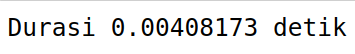
\includegraphics[width=\linewidth]{img/durasi_preprocessing.png}
	\caption{Durasi menggunakan module sklearn.preprocessing.}
\end{figure}

Perangkat yang digunakan adalah Thinkpad X240, processor i5-4300u 2c/4t, ram 4gb, sistem operasi Ubuntu 18.04.


\section{Hasil}

Penerapan pada Gaussian Naive Bayes menggunakan Cross Validation.

Hasil Crossvalidation GaussianNB menggunakan dataset yang tidak menerapkan feature scaling. \\

\begin{figure}[htbp]
	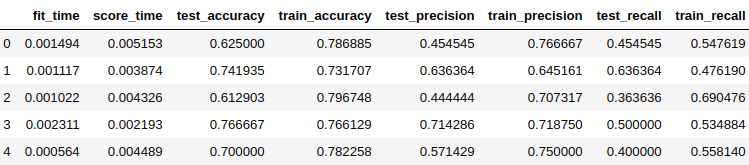
\includegraphics[width=\linewidth]{img/hasil1.png}
	\caption{Hasil Crossvalidation GaussianNB.}
\end{figure}

Rata-rata dari nilai FIT\_TIME yaitu 0.0013017654418945312 detik\\

Rata-rata dari nilai TEST\_ACCURACY yaitu sebesar 0.6893010752688171\\

Rata-rata dari nilai TEST\_PRECISION yaitu sebesar 0.5642135642135642\\

\begin{figure}[htbp]
	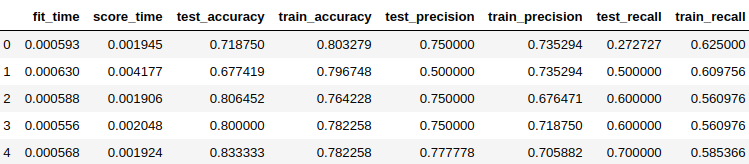
\includegraphics[width=\linewidth]{img/hasil2.png}
	\caption{Hasil Crossvalidation GaussianNB.}
\end{figure}

Rata-rata dari nilai FIT\_TIME yaitu 0.0005871295928955078 detik\\

Rata-rata dari nilai TEST\_ACCURACY yaitu sebesar 0.7671908602150537\\

Rata-rata dari nilai TEST\_PRECISION yaitu sebesar 0.7055555555555555\\

\section{Kesimpulan}

Berdasarkan pengujian tersebut, dapat disimpulkan bahwa penggunaan MinMaxScaler untuk feature Glucose pada dataset PIMA INDIAN menghasilkan rata-rata waktu training lebih cepat 45\%, akurasi 11\% lebih tinggi, dan precision 25\% lebih tinggi dibanding tiidak menggunakan MinMaxScaling pada pengujian cross validation dengan menggunakan model Gaussian Naive Bayes.

\begin{thebibliography}{00}
\bibitem{b1} Wikipedia. \textit{``Feature scaling,''}. (Online). (\path {https://en.m.wikipedia.org/wiki/Feature_scaling}). Diakses pada 27 September 2019
\end{thebibliography}

\end{document}
